\chapter{Comparing Algorithms}


% it 1
With the {\tt norMmix} package explained, we can turn to comparing it to 
existing methods. As previously stated, the implementation representing the 
EM-algorithm is the {\tt mclust} package. It will be used with very little 
deviation from out-of-the-box settings, safe for restriction of the covariance 
models. This is done, so we can compare like with like.
The specific command that performs the EM-algorithm is:

\begin{Schunk}
\begin{Sinput}
>     mclust::Mclust(x, G=cl, modelNames=mo)$BIC
\end{Sinput}
\end{Schunk}

Where {\tt cl} is a vector of integers of however many components we are trying 
to fit and {\tt mo} are the model names:

\begin{Schunk}
\begin{Soutput}
 [1] "EII" "VII" "EEI" "VEI" "EVI" "VVI" "EEE" "VEE" "EVV" "VVV"
\end{Soutput}
\end{Schunk}

The {\tt \$BIC} element of the results is taken as the main tool for model 
selection, as it is advertised in the package authors paper \cite{Scr16}.

There is however a small but crucial change applied to these results.
The {\tt mclust} package authors have flipped the definition of the BIC to mean:
\begin{equation} 
    2 ln(\hat{L}) - ln(n) \#\{par\}
\end{equation}
instead of the more common
\begin{equation} 
    ln(n) \#\{par\} - 2 ln(\hat{L})
    \label{eqn:BIC}
\end{equation}
Where $n$ is the number of observations, \#\{par\} is the cardinality of the 
parameter vector and $\hat{L}$ is the estimated log-likelihood.

So, even if not explicitly mentioned, we use the negative of the values returned
by {\tt mclust}.

Another thing that should be stated before all else is the difference in 
initialization between {mclust}'s pre-clustering and CLARA. CLARA is dependent
on random number generators. As such, unless a fixed seed is chosen, every 
iteration of CLARA will return a different result. Unlike {\tt mclust}, which 
will, for given data, always return the same results. The effect on the 
following findings is that results will spread out for data obtained from 
CLARA results.

First, we illustrate the structure of the graphical results we will be 
presenting hereafter. The basic shape of the plots will be the BIC value 
plotted against the number of components. This is in line with {\tt mclust}'s
manner of visualizing data, however since our method is to some extent RNG 
dependent, we are forced to display multiple runs of the algorithm on the same
graph. Therefore we split the plot according to covariance model, putting 10
models in 10 graphs in a plot. Here an example:


\begin{figure}[h!]
    \begin{Rgraph}[0.9]
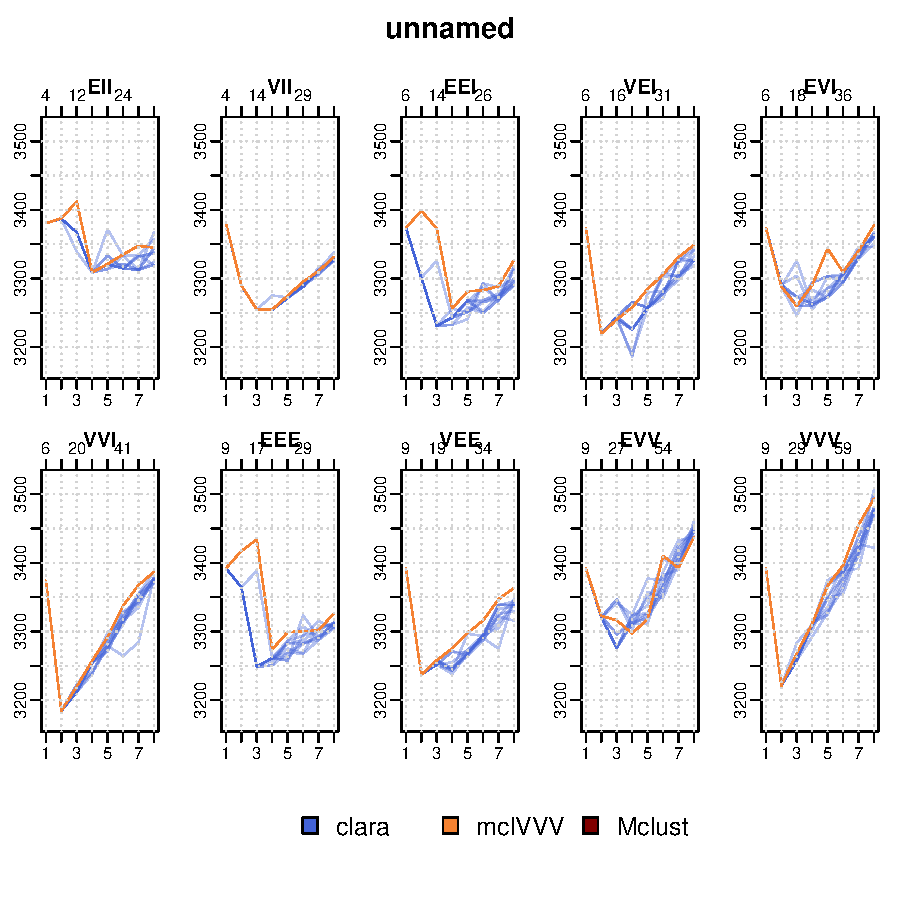
\includegraphics{chapter3-bicplotdemoplot}
    \caption{Example of comparison plot}
    \label{fig:ExPlot}
    \end{Rgraph}
\end{figure}

As can be seen from the formula of the BIC value \ref{eqn:BIC}, lower is better.
When selecting a model based on BIC, we take the model and component with the 
lowest value to be the best fitting model. Although this may not necessarily
the 'correct' model, that is, the model from which the data arises.

There are many ways in which this type of model selection might miss the 
correct model, for example by 'gluing together' multiple components into one,
or covering the dataset in a 'patchwork' of smaller components, to name a few.
We will discuss them as they arise in the following analysis of simulations.

The simulations were set up very simply. An \Rp script was written and in each
the {\tt norMmix} package is loaded, the datasets are defined and {\tt fitnMm}
was applied a number of times. An example script can be found in the appendix
\ref{App:sims}.

A few things of interest are what happens:

\begin{itemize}
    \item To time needed for the simulation
    \item When we vary the sample size of the data sets.
    \item When the generating mixture is 'difficult'.
    \item When the data does not arise from a normal mixture.
\end{itemize}

The data used here should have been provided along with this thesis in digital 
form in a folder called {\tt /simulations}, with individual simulations in 
their own subfolder.


\section{Time Analysis}
\label{sec:time}

The data used here is taken from the subfolder {\tt /simulations/2time}.
In this simulation we take several example mixtures and generate $n = \{500, 1000, 2000\}$.
We apply {\tt fitnMm} with {\tt clara} using ten different seeds and {\tt mclVVV}
initializations, and {\tt Mclust}.
From these, the system time was extracted and analyzed as can be gleaned from
the following code. In it, we apply \Rp's {\tt lm} function for fitting linear 
models to the times returned by the function call:

\begin{Schunk}
\begin{Sinput}
>     system.time(norMmixMLE(x, ...))[[1]]
\end{Sinput}
\end{Schunk}

We make here a choice that does not preserve any generality, as 
{\tt system.time} produces more results, that could hold important information.
However, since there is quite some measurement error to be expected as time 
approaches zero, we will content ourselves with lower expectations to the 
accuracy of the following results.


\begin{Schunk}
\begin{Sinput}
>     library(norMmix, lib.loc="~/ethz/BA/norMmix.Rcheck/")
>     # change this dir to whereever the simulations are saved
>     mainsav <- normalizePath("~/ethz/BA/Rscripts/")
>     savdir <- file.path(mainsav, "2time")
>     filelist <- list.files(savdir, pattern=".rds")
>     filelist <- grep("mcl.rds", filelist, invert=TRUE, value=TRUE)
>     f <- lapply(file.path(savdir,filelist), function(j) readRDS(j)$fit)
>     times <- unlist(lapply(f, function(j) extracttimes(j)[,,1]))
>     dims <- unlist(lapply(f, function(j) attr(extracttimes(j), "p")))
>     size <- unlist(lapply(f, function(j) attr(extracttimes(j), "n")))
>     ddims <- rep(dims, each=80)
>     ssize <- rep(size, each=80)
>     pars <- unlist(lapply(f, npar))
>     r <- lm(times ~ pars + ddims + ssize)
>     summary(r)
\end{Sinput}
\begin{Soutput}
Call:
lm(formula = times ~ pars + ddims + ssize)

Residuals:
   Min     1Q Median     3Q    Max 
-86.89  -7.45  -1.55   6.30 556.32 

Coefficients:
              Estimate Std. Error t value Pr(>|t|)    
(Intercept) -1.727e+01  8.274e-01  -20.87   <2e-16 ***
pars         9.729e-01  1.056e-02   92.16   <2e-16 ***
ddims       -3.749e+00  2.216e-01  -16.92   <2e-16 ***
ssize        9.258e-03  3.887e-04   23.82   <2e-16 ***
---
Signif. codes:  0 ‘***’ 0.001 ‘**’ 0.01 ‘*’ 0.05 ‘.’ 0.1 ‘ ’ 1

Residual standard error: 21.57 on 7916 degrees of freedom
Multiple R-squared:  0.559,	Adjusted R-squared:  0.5588 
F-statistic:  3344 on 3 and 7916 DF,  p-value: < 2.2e-16
\end{Soutput}
\end{Schunk}

The necessary time appears to be well explained by the parameter count.
The purpose of this thesis is not to conduct complexity analysis, so we will
leave it at this, satisfying our curiosity with a cursory look in figure 
\ref{fig:time}, where we plot system time against parameter length.

\begin{figure}[h!]
    \begin{Rgraph}[0.9]
\begin{Schunk}
\begin{Sinput}
>     plot(times~pars, log="xy", yaxt="n", xaxt="n", type="n")
>     legend("bottomright", legend=c("MW214", "MW34","MW51"),
+            fill=nMmcols[c(3,4,2)])
>     points(times[1:(80*30)]~pars[1:(80*30)], 
+            log="xy", yaxt="n", xaxt="n", col=nMmcols[3], pch=1)
>     points(times[(80*30+1):(80*60)]~pars[(80*30+1):(80*60)]
+            , log="xy", yaxt="n", xaxt="n", col=nMmcols[4], pch=9)
>     points(times[(60*80+1):(80*90)]~pars[(60*80+1):(80*90)], 
+            log="xy", yaxt="n", xaxt="n", col=nMmcols[2], pch=8)
>     grid()
>     sfsmisc::eaxis(1)
>     sfsmisc::eaxis(2)
\end{Sinput}
\end{Schunk}
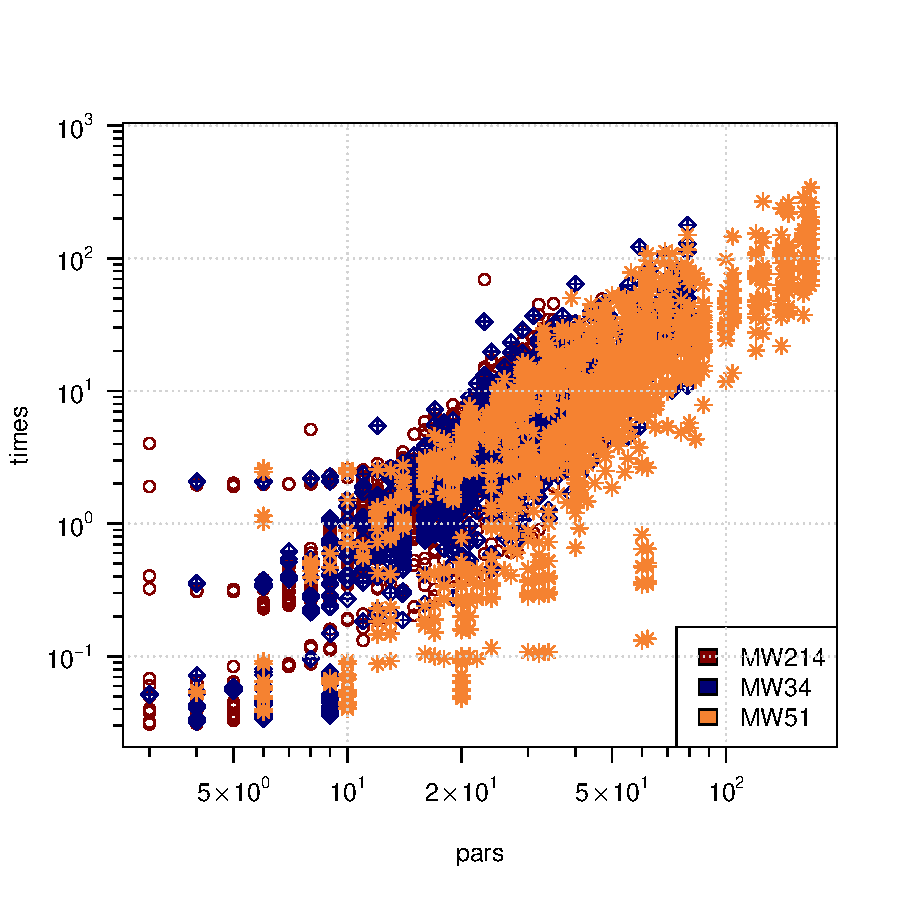
\includegraphics{chapter3-figtime}
    \caption{Log-log plot of system time against parameter length}
    \label{fig:time}
    \end{Rgraph}
\end{figure}

We can see that time is almost one to one proportional to parameter length.
It should be noted, that {\tt MW51} is a very simple mixture. It is therefore 
sensible, that MLE should find an optimum faster.

\clearpage

\section{Behaviour in {\tt n}}
\label{sec:ben}

What we would expect and like to see as we increase sample size, is a decrease
in scattering of BIC values. To that end we again use simulation data 
{\tt /simulations/2time}. In particular we show here the results of fitting to 
mixture model {\tt MW34}, shown in figure \ref{fig:MW34}. The graphs 
\ref{fig:bicmw34first} and \ref{fig:bicmw34second} show three columns
of BIC plots, each representing different sample sizes, with 
$n = \{500, 1000, 2000\}$ respectively. Furthermore, the BIC values were 
divided by the samplesize, to normalize the values to an equal scale.

\begin{figure}[h]
    \begin{Rgraph}[0.9]
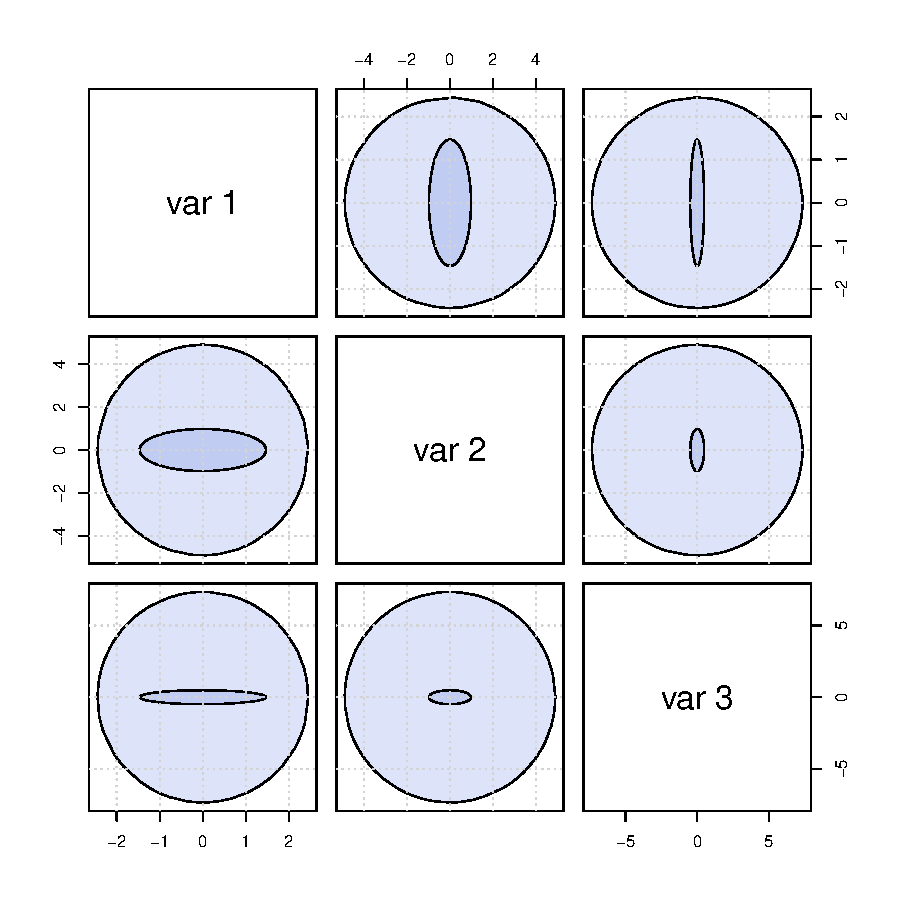
\includegraphics{chapter3-figMW34}
    \caption{The mixture model {\tt MW34}, a three dimensional, two component
             mixture with one smaller, lesser weighted component inside a 
             smaller one.}
    \label{fig:MW34}
    \end{Rgraph}
\end{figure}


\begin{figure}[h!]
    \begin{Rgraph}[0.9]
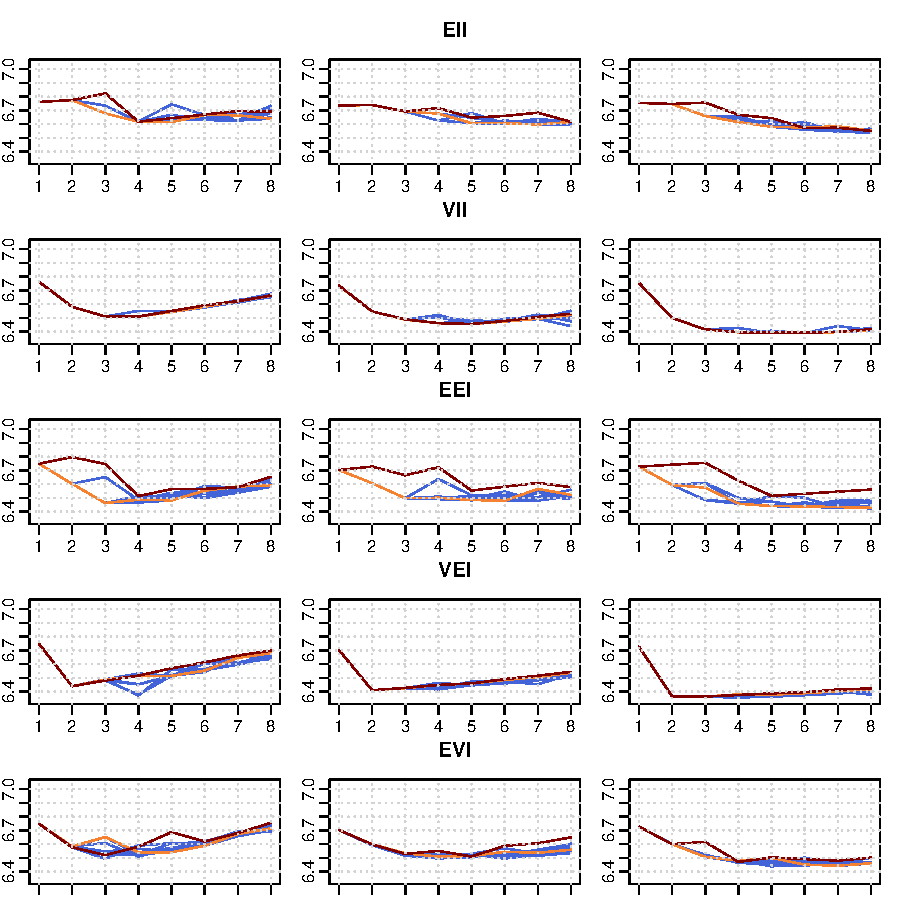
\includegraphics{chapter3-figmw34bicfirst}
    \caption{BIC values of {\tt MW34} with $n=\{500, 1000, 2000\}$. Clara was 
             applied with $10$ seeds.}
    \label{fig:bicmw34first}
    \end{Rgraph}
\end{figure}

As can be seen the desired effect is achieved. Of note are the behaviour of 
the model {\tt VEI}, where the increase in observation corrects a selection
error appearing at $n=500$. Furthermore, the correct model {\tt VVI} exhibits
a very tight grouping. The instances where {\tt mclust} is better than 
{\tt norMmix} are quite infrequent.

This type of analysis was also conducted with mixture objects {\tt MW214} and 
{\tt MW51}, but were omitted due to the lack of clear results. They are 
provided in the appendix \ref{app:ben}, with brief discussions.

\begin{figure}[h!]
    \begin{Rgraph}[0.9]
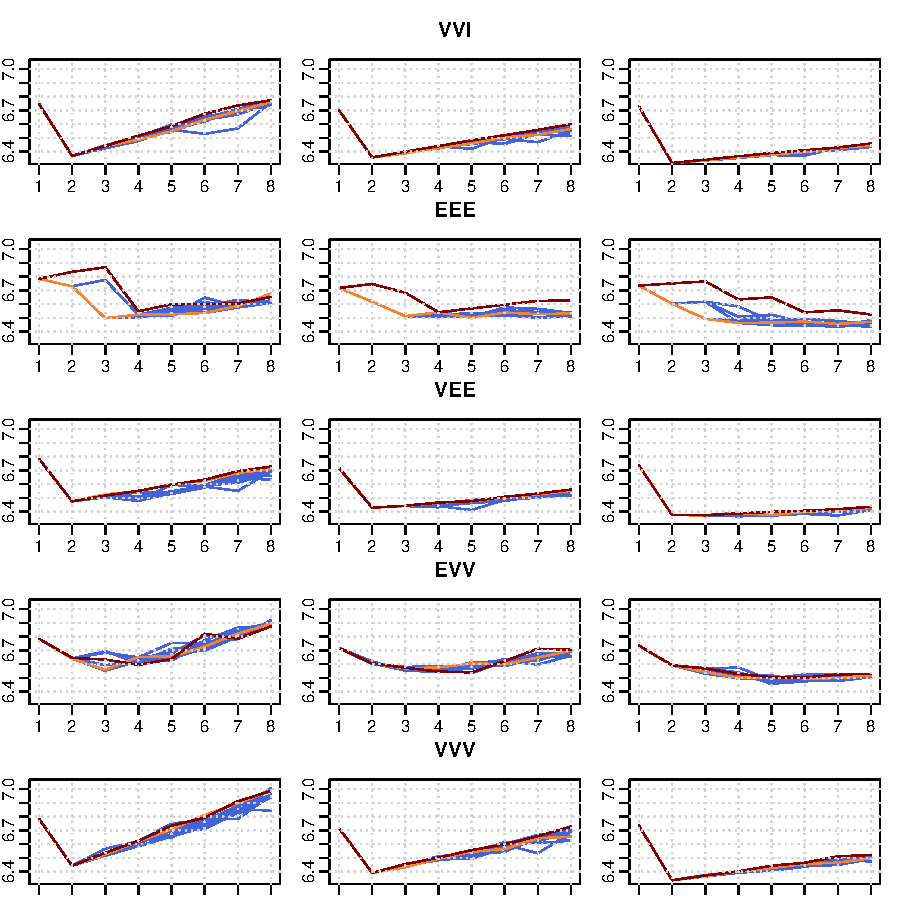
\includegraphics{chapter3-figmw34bicsecond}
    \caption{BIC values of {\tt MW34} with $n=\{500, 1000, 2000\}$. CLARA was 
             applied with 10 seeds.}
    \label{fig:bicmw34second}
    \end{Rgraph}
\end{figure}

\clearpage

\section{Difficult Mixtures}
\label{sec:dif}

In this section we analyze the two mixtures given by {\tt MW215} and {\tt MW214}.
These were generated with $n=500$ and CLARA was applied $50$ times.
These are a trimodal and a claw-like distribution. These types of mixtures were 
also discussed in \cite{Mar92}, in the univariate case, where they proved to be 
difficult to fit.

First the trimodal mixture shown in figure \ref{fig:MW215}. The difficulty 
lies in the components of various sizes lying close together.

\begin{figure}
\begin{Rgraph}[0.9]
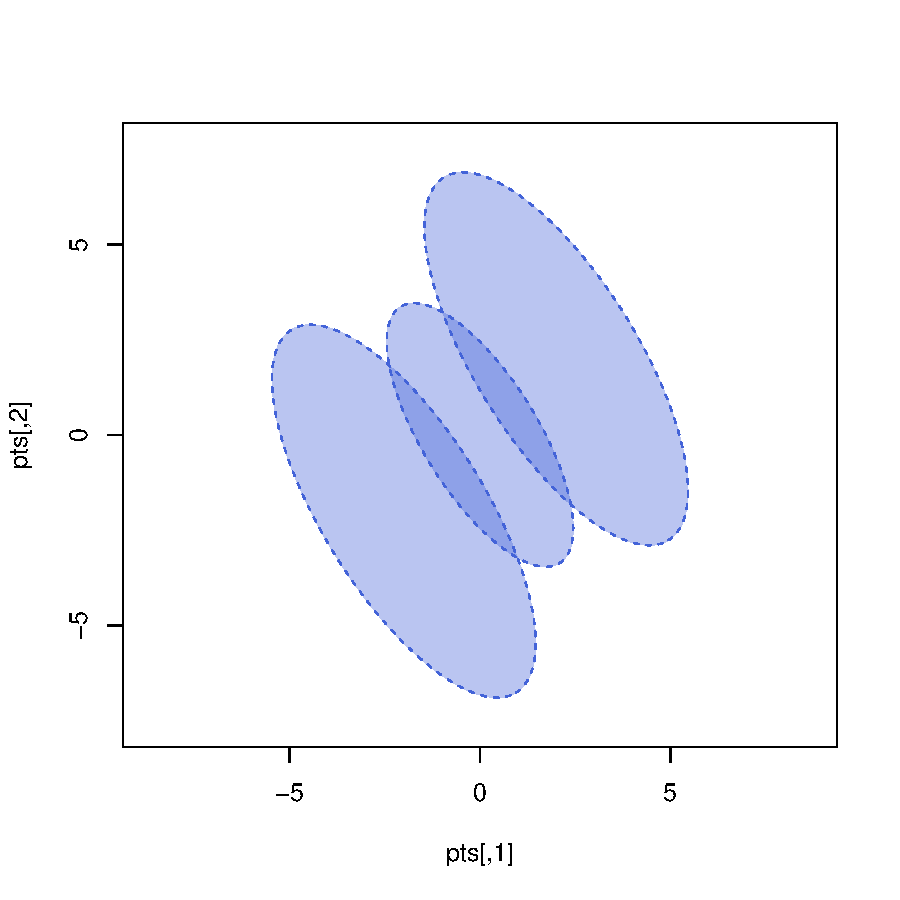
\includegraphics{chapter3-figMW215}
    \caption{Trimodal mixture {\tt MW215}. Three equally weighted, oriented, and
             shaped components of different volumes along the diagonal}
    \label{fig:MW215}
\end{Rgraph}
\end{figure}


\begin{figure}[h!]
    \begin{Rgraph}[0.9]
\begin{Schunk}
\begin{Sinput}
>     compplot(clarabic, mclbic, mclustbic, main="Fit of MW34")
\end{Sinput}
\end{Schunk}
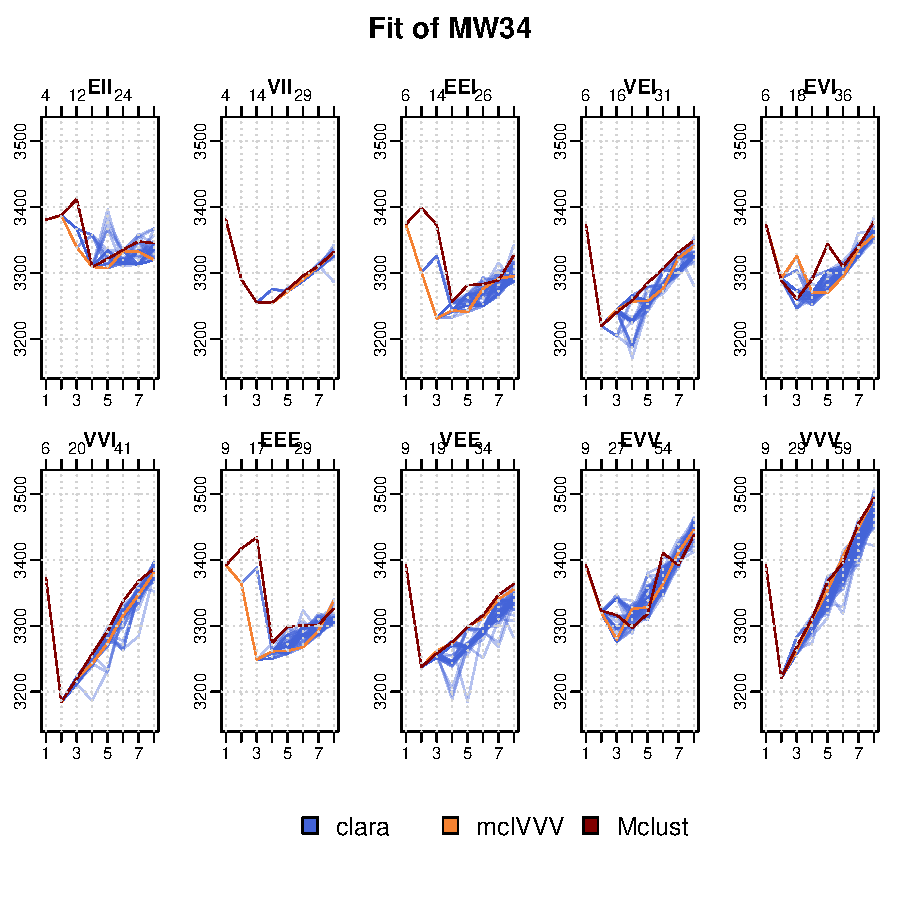
\includegraphics{chapter3-figMW34bic}
    \caption{BIC values of {\tt MW34}, correct: {\tt model="VVI", k=2}. 
             $n=500$, CLARA was applied $50$ times.}
    \label{fig:bicMW34}
    \end{Rgraph}
\end{figure}

We can see, that in many cases both initialization methods {\tt clara} and
{\tt mclVVV} manage to achieve a lower BIC value than {\tt mclust}. Although in
the case of the correct model and cluster, {\tt k=3, model="VEE"} the three 
algorithms coincide.

A search for best values reveals, that the best models selected are in almost 
all cases the correct model.

\begin{Schunk}
\begin{Soutput}
     model   count
[1,] "2 VVI" "49" 
[2,] "4 VEI" "1"  
\end{Soutput}
\end{Schunk}

The one incorrect model looks like this:

\begin{figure}[h]
    \centering
    \begin{minipage}{0.45\textwidth}
        \centering
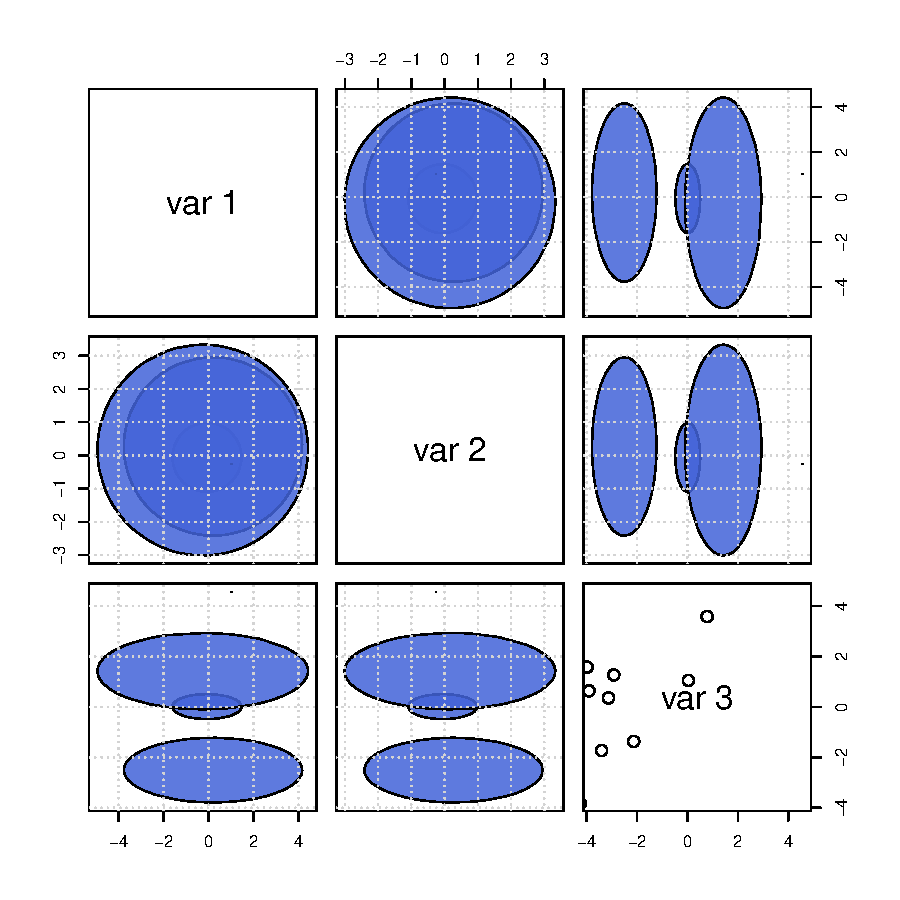
\includegraphics{chapter3-figerrorMW215}
    \end{minipage}
    \begin{minipage}{0.45\textwidth}
        \centering
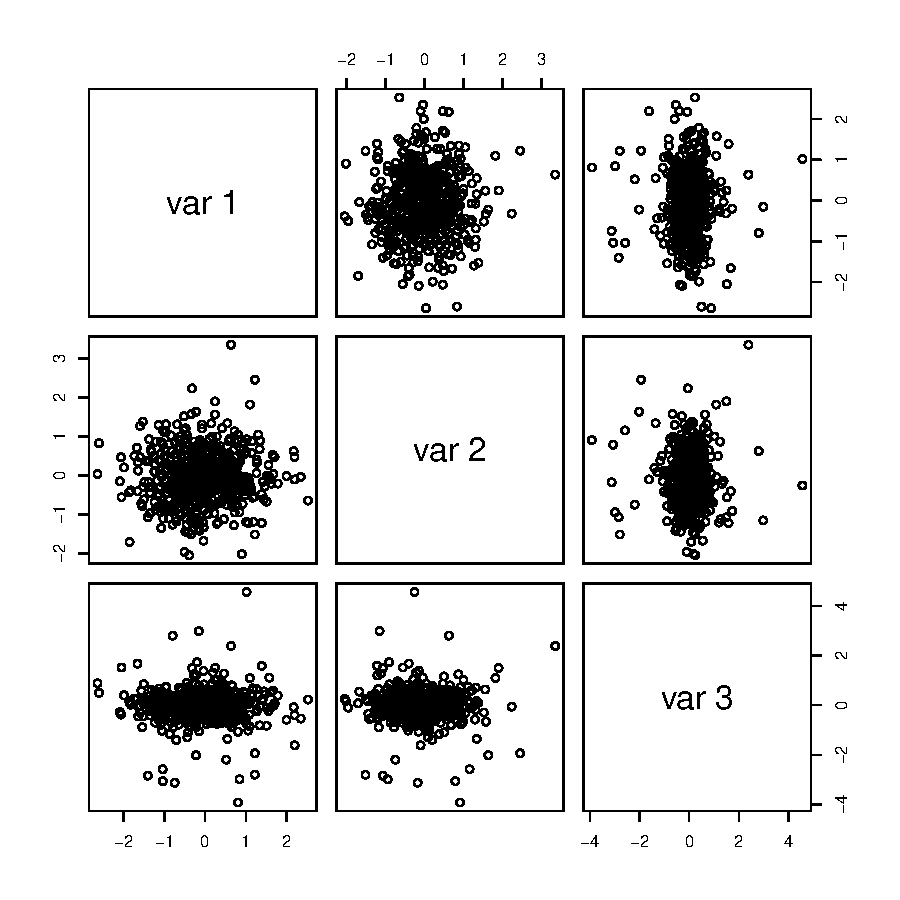
\includegraphics{chapter3-figerrorMW215x}
    \end{minipage}
\end{figure}

and has the weights: 0.942, 0.0321, 0.0244, 0.002. This is an issue of 
spurious clusters. These are clusters formed by a low number of data points
conjoined into a component with small determinant of its covariance matrix.
It is a flaw in the {\tt norMmix} package, that is not addressed.

Now for the claw-like mixture, {\tt MW214}. It is a mixture of six components
and a very simple {\tt "VII"} covariance model. A large encompassing component
and five smaller, lightly weighted components closely together along the 
diagonal. The inherent difficulty lies in the fact that the components overlap
and are close together as well. It is shown in figure \ref{fig:MW214}.

\begin{figure}[h!]
    \begin{Rgraph}[0.9]
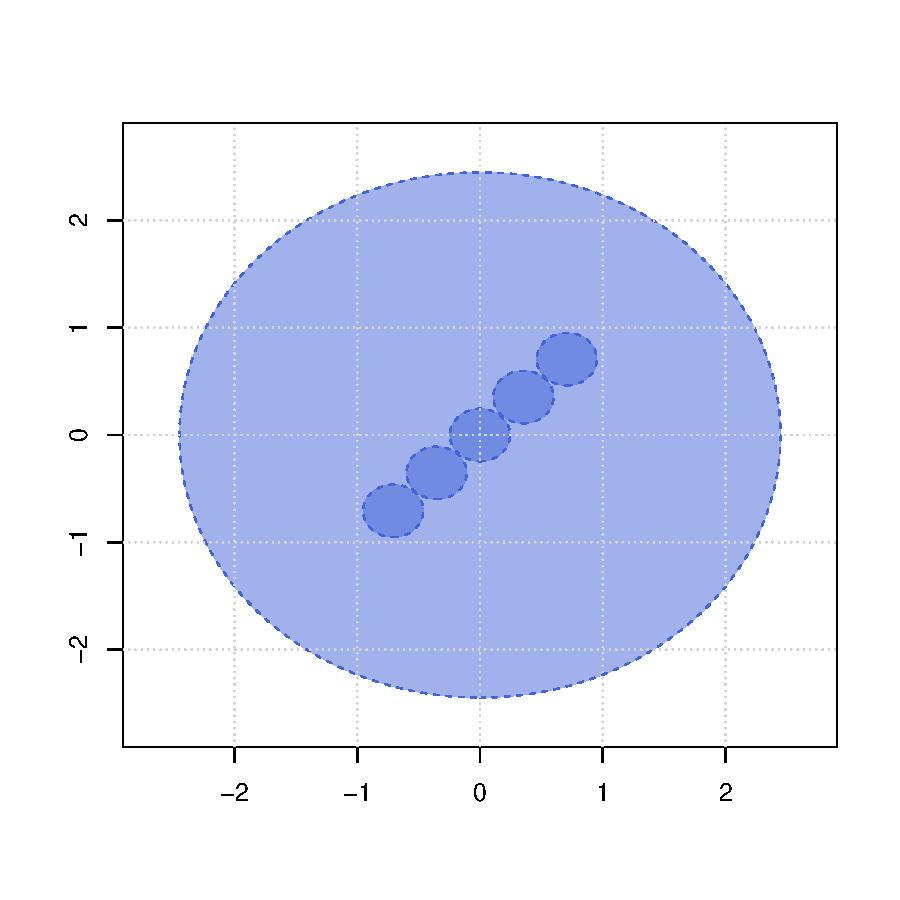
\includegraphics{chapter3-figMW214}
    \caption{Claw-like mixture {\tt MW214}}
    \label{fig:MW214}
    \end{Rgraph}
\end{figure}



\begin{figure}[h!]
    \begin{Rgraph}[0.9]
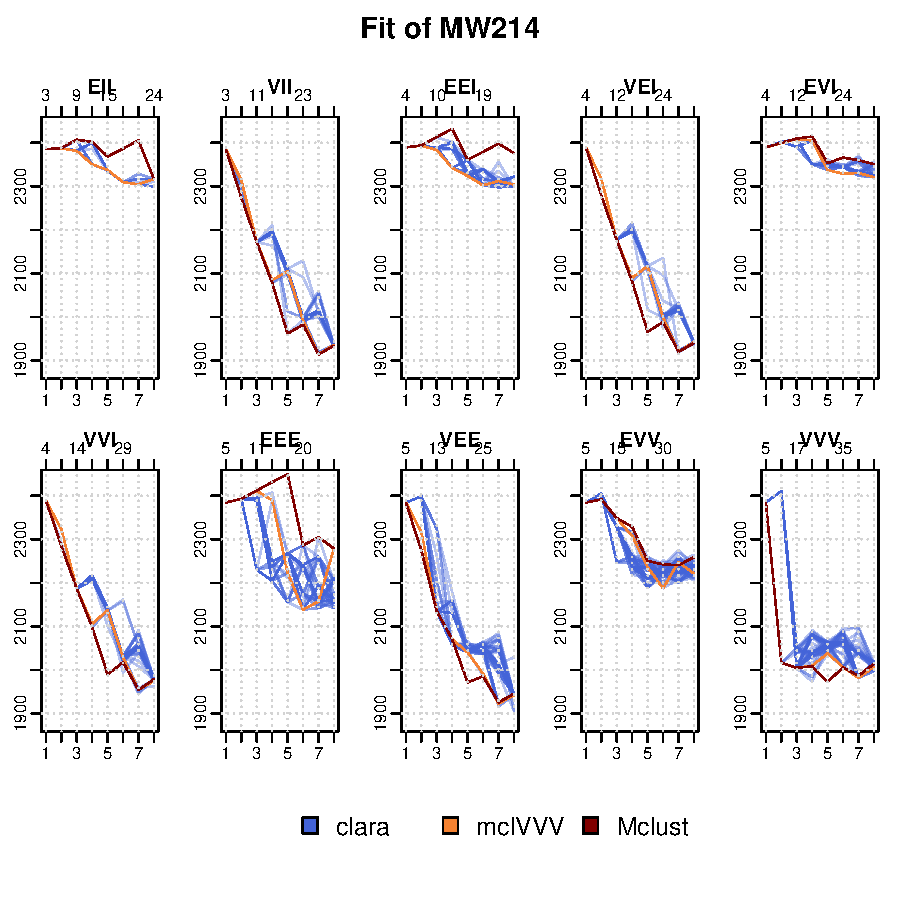
\includegraphics{chapter3-figMW214bic}
    \caption{BIC values of claw-like mixture. Best fit: {\tt model="VEE", k=8},
             correct: {model="VII", k=6}. $n=500$, CLARA was applied $50$ times.}
    \label{fig:214bis11}
    \end{Rgraph}
\end{figure}

We take a look at the best results per simulation again:

\begin{Schunk}
\begin{Soutput}
     model   count
[1,] "8 VII" "27" 
[2,] "7 VEE" "8"  
[3,] "7 VEI" "8"  
[4,] "7 VII" "4"  
[5,] "8 VEE" "3"  
\end{Soutput}
\end{Schunk}

And here are the ten best values:

\begin{Schunk}
\begin{Soutput}
      comp model BIC               
 [1,] "8"  "VEE" "1905.61014581771"
 [2,] "8"  "VEE" "1907.24944742008"
 [3,] "8"  "VEE" "1913.57109788463"
 [4,] "7"  "VII" "1913.68061849043"
 [5,] "7"  "VII" "1913.68062199219"
 [6,] "7"  "VEE" "1916.40190209225"
 [7,] "7"  "VEE" "1916.40195605402"
 [8,] "7"  "VEI" "1918.15484419568"
 [9,] "7"  "VII" "1918.35924550811"
[10,] "7"  "VII" "1918.4864952664" 
\end{Soutput}
\end{Schunk}

Here some examples of fitted mixtures:

\begin{figure}[h!]
    \begin{Rgraph}[0.9]
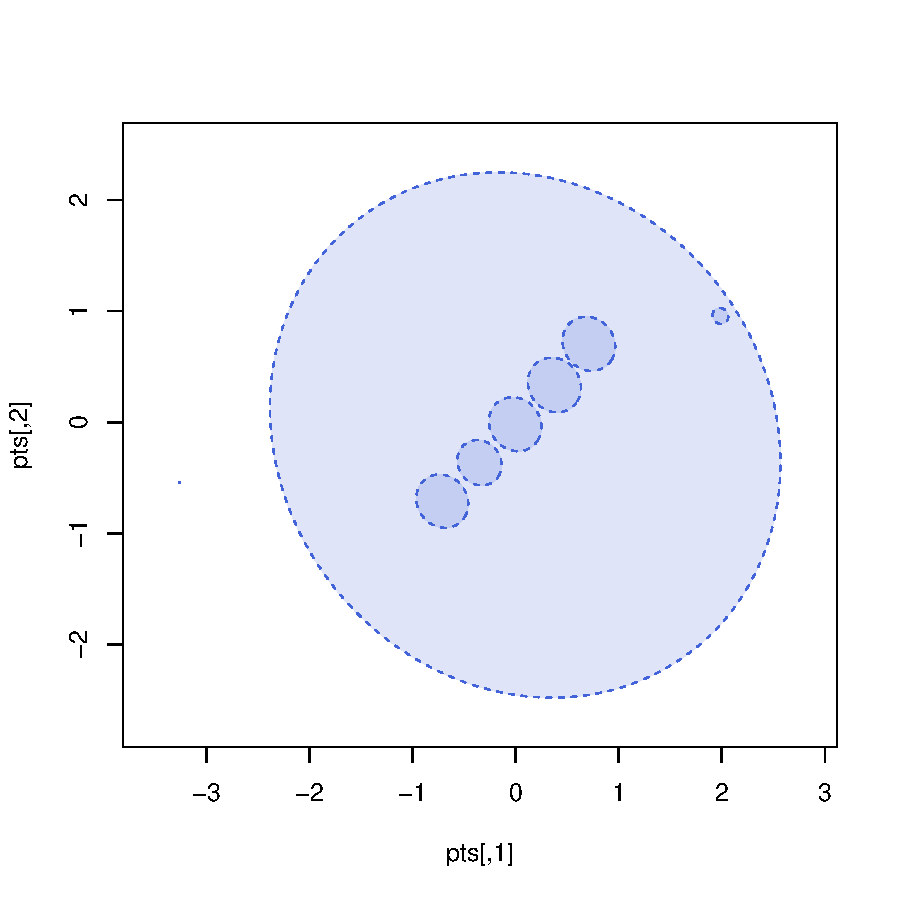
\includegraphics{chapter3-fig214fit}
    \caption{{\tt model="VEE", k=8}, correct
             model: {\tt model="VII", k=6}. Of Note Here are the Spurious 
             Clusters Appearing.}%whats n?? should be verbose
    \label{fig:MW214bestfit}
    \end{Rgraph}
\end{figure}

\begin{figure}[h]
    \begin{Rgraph}[0.9]
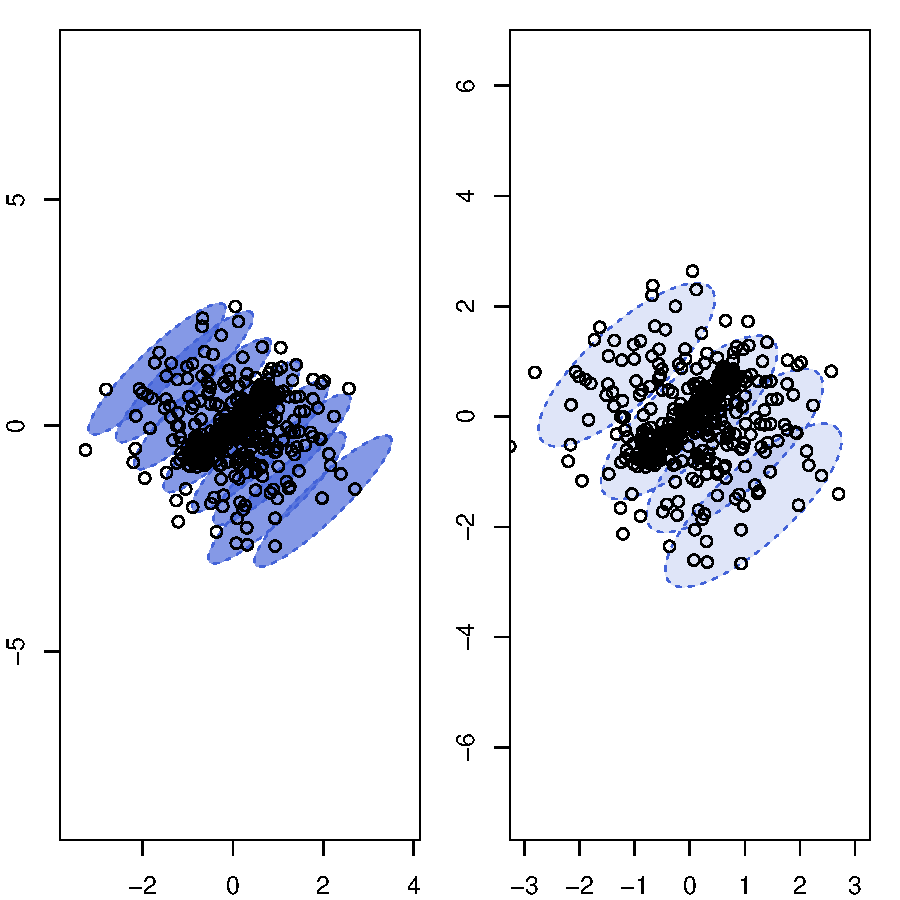
\includegraphics{chapter3-fig214fit2}
    \end{Rgraph}
    \caption{Two of the better clusters. They both follow the 'patchwork'
             covering strategy, laying patches of components over the data.}
    \label{fig:214fit2}
\end{figure}

We can see, that, subtracting the obvious hiccups of the small erroneous
components, {\tt norMmix} has correctly found the 'intended' 
distribution. This is remarkable, given the small sample size and difficulty of 
distribution. As can be seen in figure \ref{fig:214fit2}, there are mistakes in
the near best clusters, where the data is overlaid with a 'patchwork' of 
components.

\clearpage

\section{Nonnormal Mixtures}

Using only datasets generated from the intended model can hide important 
structural errors in an algorithm. To that end we also applied {\tt norMmix}
to nonnormal data to see if any erratic behaviour appears.

The data used are the {\tt SMI.12} and {\tt loss} from the package {\tt copula}
\cite{cop18}, as well as the {\tt iris} data included in base \Rp.

We begin with the {\tt SMI.12} dataset, described as "SMI.12 contains the close prices of all 20 constituents of the Swiss Market Index (SMI) from 2011-09-09 to 2012-03-28." This also doubles as high-dimensional analysis, as it is 20 dimensional.


\begin{figure}[h!]
    \begin{Rgraph}[0.9]
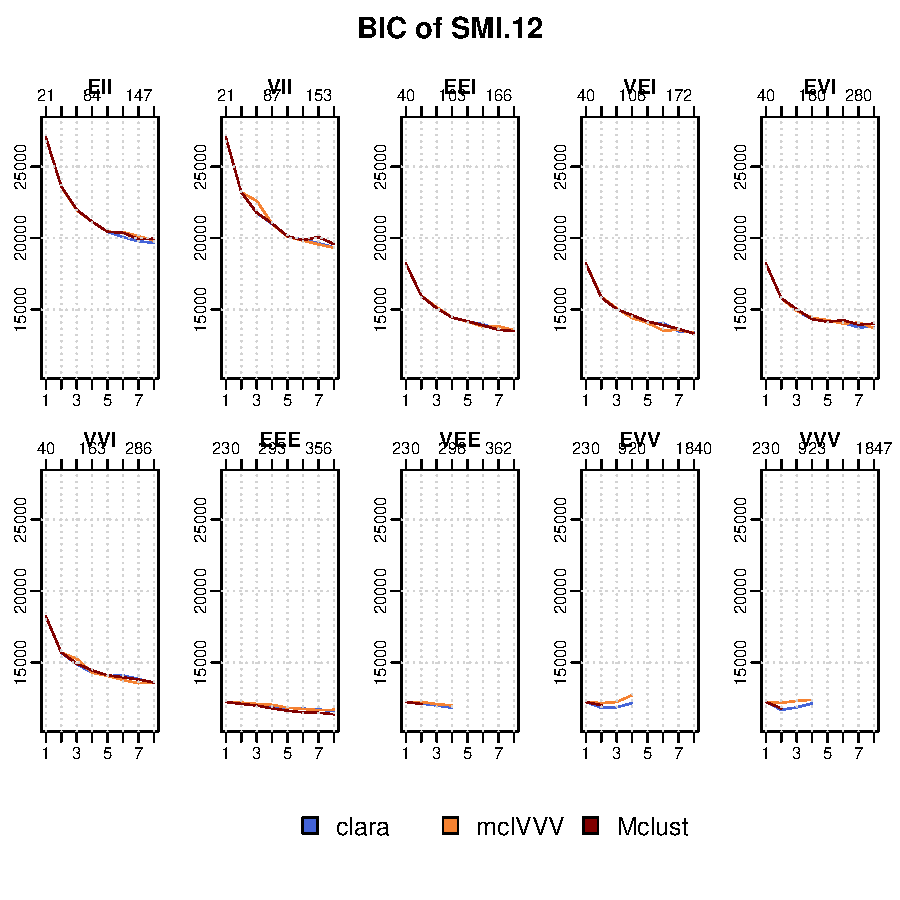
\includegraphics{chapter3-2smiplot}
    \end{Rgraph}
    \caption{The BIC values of the {\tt SMI.12} data. The blue line representing
             the {\tt clara} values is covered by the other lines. The last 
             three models are not plotted for all component sizes, as the 
             algorithm returns an error if the fitting problem is ill defined.}
    \label{}
\end{figure}

While not very spectacular, the graphs show that even at large parameter
counts our algorithm closes in on the same values as {\tt mclust}.
At these dimensions it is difficult to compare if these are actually 
equal, or even similar fits, but going by BIC values, it is at the very 
least equally viable as a working model.
The last three models are not fully plotted for all components. The reason for 
this is that {\tt norMmix} relies on {\tt mclust} in its m-step. The 
{\tt mclust} package halts computation when the clustering problem is badly 
posed. In this instance the problem is that the parameter count is much larger 
than the number of observations.

To illustrate, here are the parameter sizes for this simulation:

\begin{Schunk}
\begin{Soutput}
  EII VII EEI VEI EVI VVI EEE VEE  EVV  VVV
1  21  21  40  40  40  40 230 230  230  230
2  42  43  61  62  80  81 251 252  460  461
3  63  65  82  84 120 122 272 274  690  692
4  84  87 103 106 160 163 293 296  920  923
5 105 109 124 128 200 204 314 318 1150 1154
6 126 131 145 150 240 245 335 340 1380 1385
7 147 153 166 172 280 286 356 362 1610 1616
8 168 175 187 194 320 327 377 384 1840 1847
\end{Soutput}
\end{Schunk}

{\tt SMI.12} has 141 observations, which is exceeded by the parameter count by
all component sizes and covariance models. With a ratio of observations to 
parameters this low, it is desirable for clustering algorithms to break off and
return an error, so conclusions are not drawn from ill posed problems.

For curiosity's sake we include here the system times taken for the simulations

\begin{Schunk}
\begin{Soutput}
   models
k     EII    VII    EEI    VEI     EVI    VVI     EEE     VEE      EVV      VVV
  1 0.059  0.051  0.058  0.059   0.070  0.070   0.201   0.202    0.273    0.275
  2 0.273  0.331  1.719  1.763   4.545  3.805  61.951  59.924  224.436  232.331
  3 0.435  1.950  4.816  5.248  12.660 12.860  96.099 125.053  660.375  638.954
  4 1.384  2.456  8.715  9.145  22.173 23.065 136.370 151.448 1438.264 1556.838
  5 1.869  3.289 13.293 14.703  26.584 28.580 218.786   0.683    0.690    0.682
  6 2.703  4.125 20.578 20.490  45.355 41.667 256.036   0.010    0.011    0.022
  7 2.235  4.337 31.705 34.893  89.809 83.015 353.466   0.012    0.014    0.025
  8 3.079 13.737 63.725 44.501 110.690 98.954 396.502   0.011    0.014    0.026
\end{Soutput}
\end{Schunk}

The longest, {\tt model="VVV", k=4}, took 25.9473 minutes.


Next, we take a look at the {\tt iris} dataset with 150 observations of 4 
variables. The {\tt fitnMm} was run with $25$ different seeds. In this instance
the {\tt mclVVV} initialization was not applied, so we only compare to 
{\tt mclust}.

\begin{figure}[h!]
    \begin{Rgraph}[0.9]
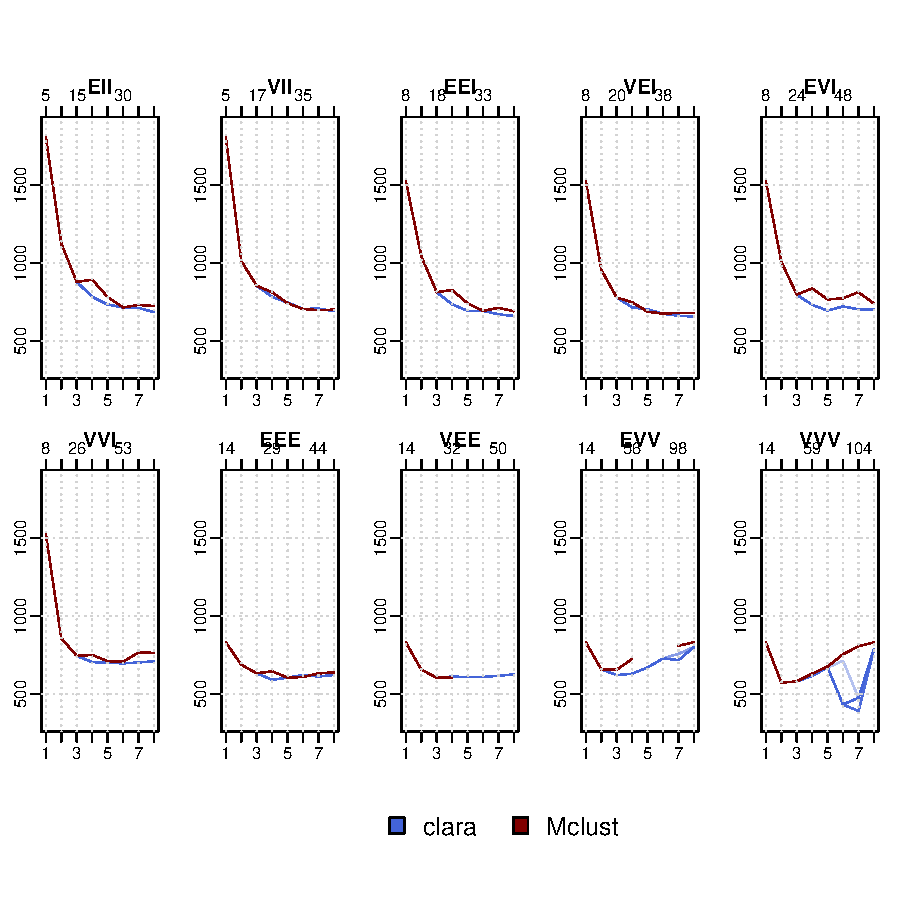
\includegraphics{chapter3-figtriris}
    \caption{The BIC values of the {\tt iris} data}
    \label{fig:triris}
    \end{Rgraph}
\end{figure}

The iris data originates from three types of plant species, which is not 
correctly identified by either {\tt norMmix} or {\tt mclust}. The best models
chosen are:

\begin{Schunk}
\begin{Soutput}
     model   count
[1,] "6 VVV" "18" 
[2,] "7 VVV" "7"  
\end{Soutput}
\end{Schunk}

Both far from three components. Furthermore {\tt mclust} does not return values
for some combinations of {\tt k} and {\tt model}. It is not clear what causes 
this, as a call to {\tt Mclust} simply returns {\tt NULL}.

Lastly, the data {\tt loss}, from the {\tt copula} package \cite{cop18}. This 
data is described as "Indemnity payment and allocated loss adjustment expense 
from an insurance company." It consists of $1500$ observations with $4$ 
variables. The BIC values are shown in \ref{fig:loss}

\begin{figure}[h!]
    \begin{Rgraph}[0.9]
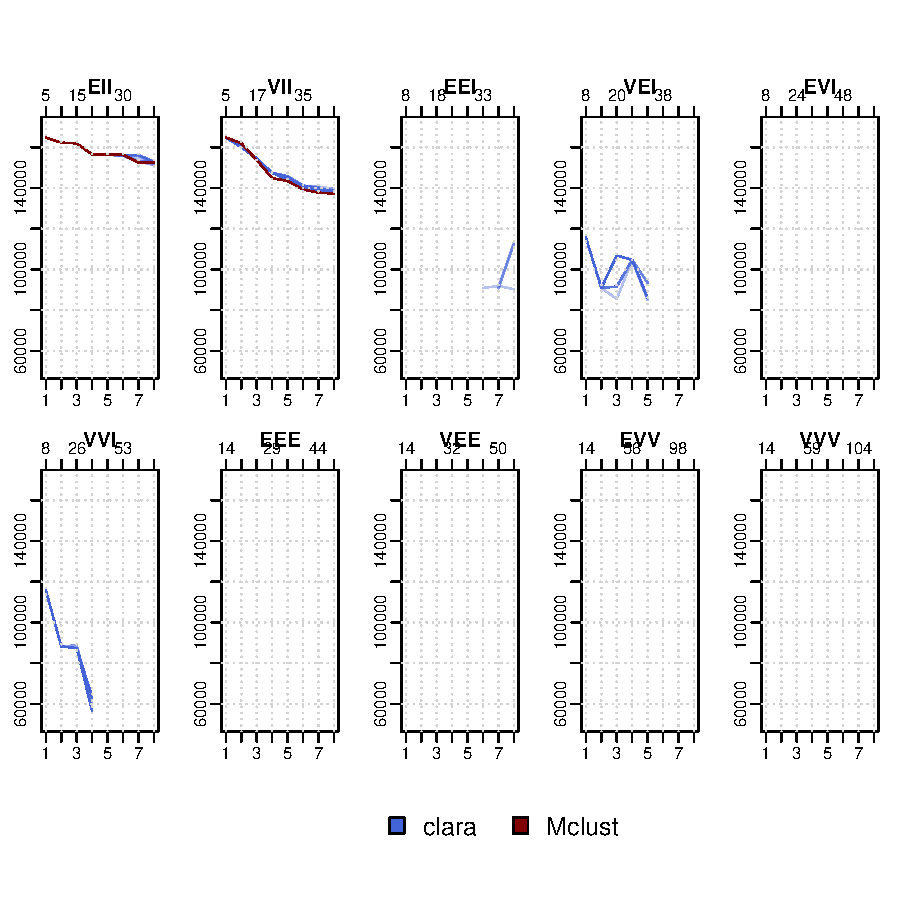
\includegraphics{chapter3-figloss}
    \caption{The BIC values of the {\tt loss}data}
    \label{fig:loss}
    \end{Rgraph}
\end{figure}

The data resists any attempt at fitting. {\tt mclust} returns {\tt NULL}, as 
with {\tt iris}. In {\tt norMmix}, the {\tt optim} function encounters an error.

\begin{Schunk}
\begin{Sinput}
>     data(loss, package="copula")
>     to <- try(norMmixMLE(loss, k=3, model="EEI"))
\end{Sinput}
\begin{Soutput}
initial  value 58082.835867 
iter  10 value 56418.201189
iter  20 value 53014.372756
iter  30 value 49490.970255
iter  40 value 46802.853871
\end{Soutput}
\begin{Sinput}
>     print(to)
\end{Sinput}
\begin{Soutput}
[1] "Error in optim(initpar., neglogl, method = method, control = control) : \n  non-finite finite-difference value [6]\n"
attr(,"class")
[1] "try-error"
attr(,"condition")
<simpleError in optim(initpar., neglogl, method = method, control = control): non-finite finite-difference value [6]>
\end{Soutput}
\end{Schunk}

